%\documentclass[a4paper,oneside,12pt]{report} % n.pag scritto in basso
\documentclass[a4paper,oneside,11pt]{book}   
% Size and sheet settings
\usepackage[a4paper, top=3.5cm, bottom=3.5cm, left=2.5cm, right=3cm, heightrounded, bindingoffset=5mm]{geometry}

% Input encoding
\usepackage[utf8]{inputenc} 
\usepackage[T1]{fontenc}
% Per gestire le immagini
\usepackage{graphicx}  
% Per inserire margini laterali
\usepackage{scrextend} 
% Per fare la title page con immagine
\usepackage{titling}  
% For special styles (code)
\usepackage[dvipsnames]{xcolor}
\colorlet{punct}{red!60!black}
\definecolor{background}{HTML}{EEEEEE}
\definecolor{delim}{RGB}{20,105,176}
\colorlet{numb}{magenta!60!black}
\usepackage{listings}

% To set depth table of contents
\setcounter{tocdepth}{4}

%% TABLES
% Utile per usare H per svuotare la cache dei floating objects come le table
\usepackage{float}     
% Necessario per rappresentare tabelle su più pagine
\usepackage{longtable} 
% Necessario per creare un nuovi tipi di colonna per le tabelle
\usepackage{array}     
\usepackage{tabu}

% Special table columns to center between cells
\newcolumntype{X}[1]{>{\centering\arraybackslash}p{#1}}
\newcolumntype{C}[1]{>{\centering\arraybackslash}m{#1}}
\newcolumntype{P}[1]{>{\arraybackslash}p{#1}}
\newcolumntype{H}[1]{>{\arraybackslash}m{#1}}

% Aggiunge funzionalità alle captions
\usepackage{caption}   
% Distacca le caption dalle table (verticalmente)
\captionsetup[table]{skip = 8pt} 
% Default: 6pt - Margine laterale  tra le celle delle tabelle
\setlength{\tabcolsep}{10pt}      
% Default: 1 - Margine verticale tra le celle delle tabelle
\renewcommand{\arraystretch}{1.7} 

% Multicolumn sections
\usepackage{multicol}

% Clickable references
\usepackage{hyperref} 
\hypersetup{
    colorlinks=true,
    linkcolor=blue,
    filecolor=black,      
    urlcolor=cyan,
    pdftitle={CLup - Implementation and Testing Document}, % Title of output file
    pdfpagemode=FullScreen,            % To open in fullscreen
}
% Command for two-part captions for tables/pictures
\newcommand{\captionit}[2]{\caption{#1}\par\begin{center}\vspace{-.01\textheight}\small#2.\end{center}}
% Command for correctly spaced coloured text
\newcommand{\red}[1]{\begingroup\color{punct}#1\endgroup}

\title{\LARGE{CLup -- Implementation and Testing Document}}
\author{Vincenzo Riccio, Giancarlo Sorrentino, Emanuele Triuzzi}
\date{February 7th, 2021}
\begin{document}

\begin{titlingpage} 
    \begin{center}
        
\includegraphics[height=0.52\linewidth]{pictures/polimi}\\ % Logo
        \begin{large}
            Software Engineering 2 \\
            A.Y. 2020-2021\\
        \end{large}
        \vspace{4cm} % Spaziatura verticale
        \begin{large} 
            \textbf{\thetitle} \\
        \end{large}
        \vspace{0.7cm}
        \theauthor
        \par\small{\url{https://github.com/SirGian99/RiccioSorrentinoTriuzzi}} \par\par
        \vspace{7.3cm} % Spaziatura verticale
        \thedate
    \end{center}
\end{titlingpage}

\newpage
\begin{table}[H]
    \begin{tabu} to \textwidth { X[0.3,r,p] X[0.7,l,p] }
        \hline
        \textbf{Deliverable:}   & ITD\\
        \textbf{Title:}         & Integration and Testing Document \\
        \textbf{Authors:}       & Vincenzo Riccio, Giancarlo Sorrentino, \newline Emanuele Triuzzi \\
        \textbf{Version:}       & 1.0 \\ 
        \textbf{Date:}          & February 7th, 2021 \\
        \textbf{Download page:} & https://github.com/SirGian99/RiccioSorrentinoTriuzzi \\
        \textbf{Copyright:}     & Copyright © 2021, Vincenzo Riccio, Giancarlo Sorrentino, Emanuele Triuzzi -- All rights reserved \\
        \hline
    \end{tabu}
\end{table}

%\href{run:../DeliveryFolder/RASD2.pdf}{Requirement Document}
%\ref{section:design_decisions}

\pagenumbering{roman}
\tableofcontents
\newpage
\pagenumbering{arabic}

\chapter{Introduction}
    \section{Purpose and scope}
    The purpose of this document is to outline the CLup prototype realized following the design proposed in the Design Document (\href{run:../DeliveryFolder/DD2.pdf}{DD}), describing the implementation and the testing activity carried out across the development. \par
    In particular, the document highlights the implemented features, the technology stack used for the development, the code structure and details on the testing phase. \par
    Furthermore, it provides the instructions to prepare a workstation configuration as close as possible to the one used during the software development and testing, in order to perfectly use and test the entire system. \par
    All the references to any software used during this phase are mentioned at the end of the document.

    \section{Definitions, acronyms, abbreviations}
    \begin{longtable}[c] { |>{\bfseries{}}C{0.25\textwidth}|H{0.55\textwidth}| }
        \hline
        \multicolumn{2}{|c|}{\textbf{Definitions, acronyms, abbreviations}} \\
        \hline
        AMS                  & Access Management System \\ \hline
        TAS                  & Turn Announcement System \\ \hline
        CLup                 & Also known as the system. It is the software to be developed. From a design-oriented point-of-view, the term is also used to refer to the mobile application, the administrative tool and the server all together \\ \hline
        Customer application & Also known as application. It is used to access the functions provided by CLup  \\ \hline
        Administrative tool  & the tool provided to store managers in order to administer stores \\ \hline
        Proxy                & The physical fallback option for customers that want to use CLup but cannot use the application. It is placed outside the store it belongs to \\ \hline
        Turn Announcement System & An external system which informs customers about who has been allowed by CLup to enter the store it belongs to \\ \hline
        Access Management System & An external system which regulates physical entrances and exits to the store it belongs to by interacting with CLup \\ \hline
        App-customer & A customer who uses CLup functions through the application \\ \hline
        Proxy-customer & A customer who uses CLup functions through the proxy \\ \hline
        User & Either a customer or a store manager \\ \hline
        Long-term customer & With respect to a certain store, a customer who already used CLup to visit it \\ \hline
        Current occupancy & Also known as occupancy. It can be referred to the store or one of its sections. For the store, it is the number of people inside it. For the product sections, it is an index of the approximate number of people inside it the system can be aware of \\ \hline
        Maximum occupancy & Refers to the store or one of its sections. It is the maximum number of people allowed to be in that area \\ \hline
        Virtual queue & Also known as access queue or simply queue. It represents the set of customers who lined up through the app or the proxy \\ \hline
        Line-up & With respect to a customer and a store, it is the event of joining the queue \\ \hline
        Visit request & A customer’s request to visit a store. It can be either a line-up request or a booking request \\ \hline
        Line-up request & A request made by the customer to line-up for a store \\ \hline
        Booking request & A request made by the customer to book a visit to a store \\ \hline
        Visit & The realization of a visit request which takes place when a customer enters the store. After the customer exits the store, we talk about completed visit, otherwise it is a visit in progress  \\ \hline
        Visit token & A unique token bound to a visit request. It allows the Customer to enter and exit the store \\ \hline
        Pending request & A customer’s visit request that does not have a visit associated with and is not allowed to enter the store it is associated with \\ \hline
        Ready request & A customer’s visit request that does not have a visit associated with and is allowed to enter the store it is associated with \\ \hline
        Fulfilled request & A customer’s visit request that has an associated visit in progress \\ \hline
        Completed request & A customer’s visit request that has an associated completed visit \\ \hline
        Active request & A customer’s visit request that is not a completed request (thus it is either a pending, a ready or a fulfilled request) \\
        \hline
    \caption{Definition, acronyms, abbreviations}
    \label{table:definitions_acronyms_abbreviations}
    \end{longtable}

    \section{Revision history}
    1.0 -- First version of the document (February 7th, 2021).
    
    \section{Reference documents}
    \begin{itemize}
        \item I\&T Assignment A.Y. 2020-2021;
        \item \href{run:../DeliveryFolder/RASD2.pdf}{CLup Requirements Analysis and Specification Document};
        \item \href{run:../DeliveryFolder/RDD2.pdf}{CLup Design Document};
        \item Teaching material provided by professors Matteo Rossi and Elisabetta Di Nitto.
    \end{itemize}

    \newpage
    \section{Document structure}
    The reference structure used for the document is an adapted version of the one suggested by professor Matteo Rossi of Politecnico of Milan.

    \subsubsection{Chapter 1} 
    Chapter 1 is an introduction to the implementation and testing of the software presented in the Requirement Analysis Specification Document and the Design Document.
    
    \subsubsection{Chapter 2} 
    Chapter 2 defines the implemented functionalities of the system.

    \subsubsection{Chapter 3} 
    Chapter 3 focuses the analysis on the adopted programming languages, frameworks and external APIs used to implement the system and to perform the testing.

    \subsubsection{Chapter 4} 
    Chapter4 describes the source code structure of both the Server and the mobile applications.

    \subsubsection{Chapter 5}
    Chapter 5 provides information on how the testing has been performed and its outcome. 

    \subsubsection{Chapter 6}
    Chapter 6 contains a list of instructions to install the mobile applications, the JavaServer and to configure the database.

    \subsubsection{Chapter 7}
    Chapter 7 contains a report on the effort spent by all the members of the group while writing the current document.
    
    \subsubsection{Chapter 8}
    Last chapter contains references to the tools and resources used to implement the system and to write the document.

\chapter{Implemented functions}
    \section{Overview}
    The developed prototype focuses on the customers' use cases outlined in the RASD, although simplified. It includes:
    \begin{itemize}
        \item a fully-implemented database schema, including a test instance;
        \item a server providing part of the designed functionalities;
        \item an iOS mobile application for the customer;
    \end{itemize}
    Thus, the provided functionalities are the following:
    \begin{itemize}
        \item allow customers to line up for a desired store;
        \item allow customers to book a visit for a desired store;
        \item allow customers to cancel a request they made;
        \item register a mobile application;
        \item retrieve the active requests of a customer;
        \item retrieve chains and stores of a specified city
        \item manage entrances of a customer;
        \item manage exits of a customer;
        \item automatic state changing for line up requests;
        \item scheduling of automatic state changing for booking requests;
        \item check the current occupancy constraints of the store;
        \item provide a raw estimation of the queue disposal time of a store;
        \item provide a raw estimation of the estimated time of entrance of a lineup request.
    \end{itemize}
    The server prototype does not foresee the functionality described in the DD which changes the access policy of each store taking into consideration which of the two different “zones” the store is in (the yellow and green one). For the sake of simplicity of the prototype, stores are considered always in the “green zone”.  \par
    Also, the prototype does not focus on the performance or on the  software system attributes identified in the RASD, since it is intended only to demonstrate the main CLup functionalities.

    \section{Requirements achieved}
    The implemented prototype satisfies most of the functional and nonfunctional requirements presented in the \href{run:../DeliveryFolder/RASD2.pdf}{CLup Requirements Analysis and Specification Document} (RASD) and the \href{run:../DeliveryFolder/DD2.pdf}{Design Document} (DD).
    
    \subsubsection{Functional requirements}
    \begin{itemize}
        \item The system shall allow managers to monitor entrances (R2);
        \item The system shall allow managers to monitor exits (R3);
        \item The system shall authorize accesses to the store (R4);
        \item The system shall authorize customers to enter if and only if the store would not exceed the maximum number of people allowed inside it (R4.1);
        \item The system shall provide a way to line-up in the virtual queue of the store (R5);
        \item The system shall provide a way to exit the queue before entering the store (R6);
        \item The system shall provide the possibility to book a time interval for visiting the store (R8);
        \item The system must not allow customers to book a visit in a time interval if, over its duration, bookings by other users already maximize store occupancy (R9);
        \item When booking a visit, the system shall allow customers to specify what kind of products they intend to buy (R10);
        \item The system shall provide the possibility to cancel a booked visit before entering the store (R11);
        \item The system shall inform customers when they are allowed to enter the store (R19);
    \end{itemize}
    
    \subsubsection{Non-functional requirements}
    \begin{itemize}
        \item The application should be easy to use (NF10);
        \item CLup shall give priority to booking requests over line-up requests (NF11);
        \item Customers can remotely line-up in a store’s queue only if they are not in the queue of any store at that moment (NF12);
        \item Customers can book a visit to a store for a specific time interval only if they have not booked any other visit which overlaps with that time interval (NF13);
        \item Customers can book a visit to a store for a specific time interval only if it starts after the current queue disposal time of that store (NF14).
    \end{itemize}
    
\chapter{Adopted frameworks}
    This section better delve into the technology stack outlined in the Design Document. The design decisions omitted in this chapter are retrievable from the  \href{run:../DeliveryFolder/DD2.pdf}{Design Document}.
    \section{iOS Mobile application}
    The mobile application logic has been developed in Swift, an powerful and intuitive programming language designed by Apple. Meant as an alternative to Objective-C, and up to 2.6 times faster than it, in recent years it has become the main programming language for iOS and macOS applications. To build the UI, the chosen framework is SwiftUI, which offers a declarative way to build user interfaces with few lines of code. It is developed by Apple itself and thus it is designed for Swift and Apple devices. \par
    Furthermore, SwiftyJSON was used for easy managing of JSONs.
    
    \section{Java Server}
    The server has been implemented using Apache TomEE, which combines different Java Enterprise projects used to satisfy the requirements:
    \begin{itemize}
        \item \textit{Apache Tomcat}: HTTP server and Servlet container supporting Java Servlet;
        \item \textit{Apache OpenEJB}: Open-source Enterprise JavaBeans (EJB) container system. Enterprise JavaBeans is a server-side software that encapsulates business logic of the server application;
        \item Apache OpenJPA: Open-source Java Persistence API (JPA) 2.1 implementation. \par
        JPA is a Java EE application programming interface specification that describes the management of relational data in enterprise Java applications. Persistence in this context covers three areas:
            \begin{itemize}
                \item the API itself, defined in the \texttt{javax.persistence} package;
                \item the Java Persistence Query Language (JPQL), which queries against entities stored in a relational database. Queries resemble SQL queries in syntax, but operate against entity objects rather than directly with database tables;
                \item object/relational metadata.
            \end{itemize}
        The interfaces between the presentation layer and the application layer are designed according to the REST (Representational State Transfer) architectural style and are based on the HTTP protocol. Thus, each interaction between those layers is stateless and follows a client-server approach. \par
        Each resource is identified by a URI and the transferred data are represented using the JSON standard. 
    \end{itemize}
    
    \subsection{EclipseLink}
    Since JPA is only a specification, a Persistence Provider is needed to implement the Object Relational Mapping. The chosen provider for this purpose is Eclipselink.

    \subsection{JAX-RS API}
    JAX-RS is part of the Java EE specification and is designed to simplify the development of RESTful applications. It consists of a set of interfaces and annotations defined in the javax.ws.rs package.
    
    \subsection{Apache Maven}
    As Maven is perfectly integrated in IntelliJ IDEA, it has been used as software project management tool to manage the dependencies and the lifecycle of each module. \par
    Each module, better detailed in the next section, is described by its own pom.xml, which is the Maven project object model (POM) descriptor. It is an XML file that contains information about the project and configuration details used by Maven to build the project.
    \subsection{org.json}
    Also known as “\textit{JSON-Java}”, it is one of the most popular libraries used to deal with JSON (JavaScript Object Notation) in Java. It also includes the capability to convert between JSON and XML, HTTP headers and more. It is used to parse (resp. prepare) the request (resp. response) which is received (resp. sent) by the RESTful servlets.
    \begin{itemize}
        \item \textit{JSONObject}: similar to Java’s native Map object, where keys are Strings that cannot be null and values are anything from Boolean, Number, String, JSONObject or JSONArray, or null;
        \item \textit{JSONArray}: it is an ordered collection of values, resembling Java’s native Vector implementation.
    \end{itemize}
    The main methods used are:
    \begin{itemize}
        \item \texttt{put(key: \red{String}, value: \red{Object})}: inserts in the JSONObject the field specified;
        \item \texttt{put(element: \red{Object})}: appends the element to the JSONArray;
        \item \texttt{get(key: \red{String})}: gets the object associated with the supplied key, throws JSONException if the key is not found.
    \end{itemize}

    \subsection{JUnit and Mockito}
    JUnit5 is the tool chosen in order to perform unit and integration testing. 
    The tool is perfectly integrated with Maven and IntelliJ IDEA and serves as a foundation for launching testing frameworks on the JVM. In particular, JUnit has been used together with the Mockito framework, which allows to perform scaffolding, defining specific stubs whenever the components under test cannot be tested in isolation. 
\chapter{Code structure}
    \section{iOS Mobile application}
    The mobile application code is organized as follows:
    \begin{itemize}
        \item the \textbf{Model} folder contains what is needed to model the data received from the server and to make them available to the entire application;
        \item the \textbf{Views} folder contains the pure frontend part of the mobile application, the SwiftUI views;
        \item the \textbf{Assets.xcassets} folder and the \textbf{LaunchScreen.storyboard} file gather the static data which are shown in the user interfaces or at the launch of the app 
        \item \textbf{SwiftyJSON.swift} contains the homonym framework used to deal with JSONs;
        \item \textbf{Extensions.swift} and \textbf{ViewExtensions.swift} contain our extensions of the classes/structures provided by Swift and SwiftUI;
        \item \textbf{Routes.swift} contains the needed endpoints of the RESTful API offered by the server;
        \item \textbf{CLupApp.swift} is the app main file, according to the SwiftUI lifecycle;
        \item \textbf{SIController.swift} contains the controller of the interactions with the server.
    \end{itemize}

    \begin{figure}[H]
        \centering
        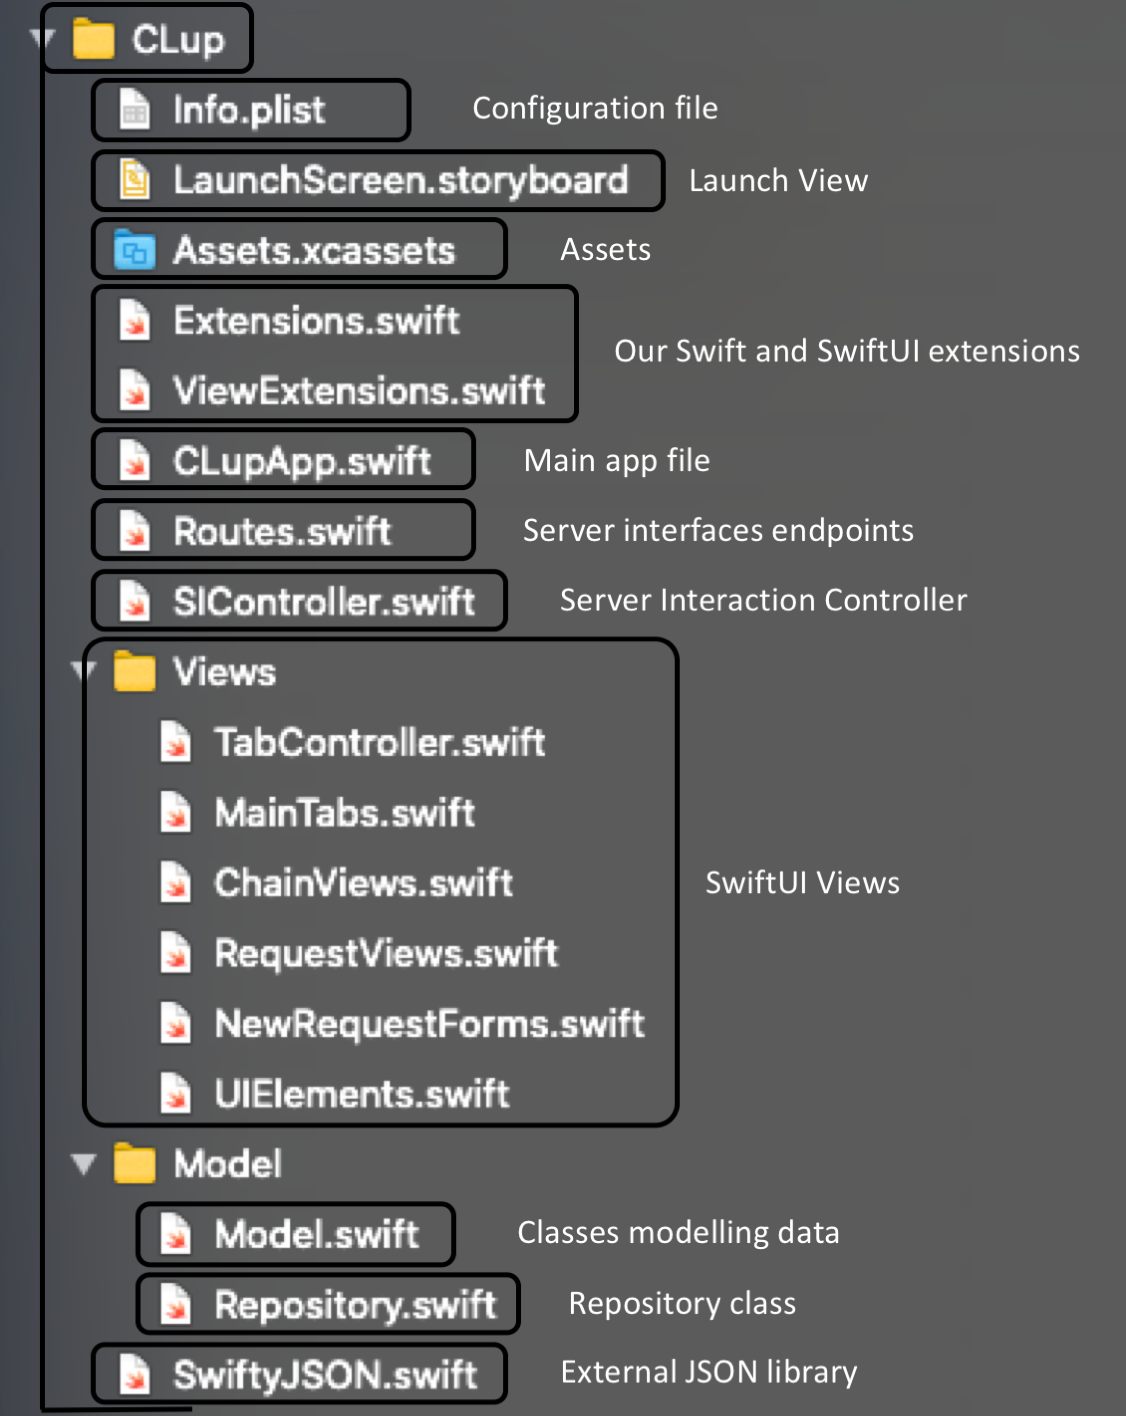
\includegraphics[width=.8\textwidth, height=\textheight, keepaspectratio]{pictures/codestructure_swift.png}
        \caption{Code structure of the mobile application}
        \label{figure:codestructure_swift}
    \end{figure}
    
    
    \section{Java Server}
    At the highest level, the source code is organized in three base modules, which implement the internal server components, plus a module for the integration testing:
    \begin{itemize}
        \item \textbf{BusinessModule}: following the design document guidelines, it includes the following subcomponents as different stateless JavaBeans:
        \begin{itemize}
            \item \textbf{CustomerController}: this component s in charge of retrieving and providing customers with their information, such as their active line-up and booking requests;
            \item \textbf{RequestHandler}: this component is the one in charge of collecting customers’ visit requests, accepting or rejecting them, and of cancelling the same requests whenever the customer who placed them asks for it;
            \item \textbf{StoreStatusHandler}: this component is the one in charge of providing all the information concerning the stores managed by CLup, such as their opening time, their current occupancy, their product sections and relative occupancies, their current queue disposal time;
            \item \textbf{VisitManager}: this component is the one in charge of coping with visits and visit requests to the stores managed by CLup. In fact, it regulates the order in which customers are allowed to visit the stores they made visit requests for. The VisitManager also provides an interface to allow entrances and exits to the stores managed by CLup, by checking if, given a visit token and a store, the token is associated with a visit request in ready state for the selected store.
        \end{itemize}
        \item \textbf{DataModel}: it is the module containing the homonym bean and the entities (classes) which map the database tables. It defines the data model of the system and interacts, thanks to JPA, with the DBMS in order to ensure data persistence. All the other components of the system interact with the stateless DataModel bean, which is the only one in charge of dealing with the persistence context. It contains the JPA descriptor (\texttt{persistence.xml}).
        \item \textbf{REST-API}: it is the module which, following the design document guidelines, contains the servlets offering the interfaces mentioned in the DD. It contains the classes managed by the JAX-RS framework and which interact with the beans of the BusinessModule to offer the requested service. 
        \item \textbf{IntegrationTestingModule}: it is the module used to perform the integration testing of the previous ones. More details are provided in the section concerning the integration testing.
    \end{itemize}
    \begin{figure}[H]
        \centering
        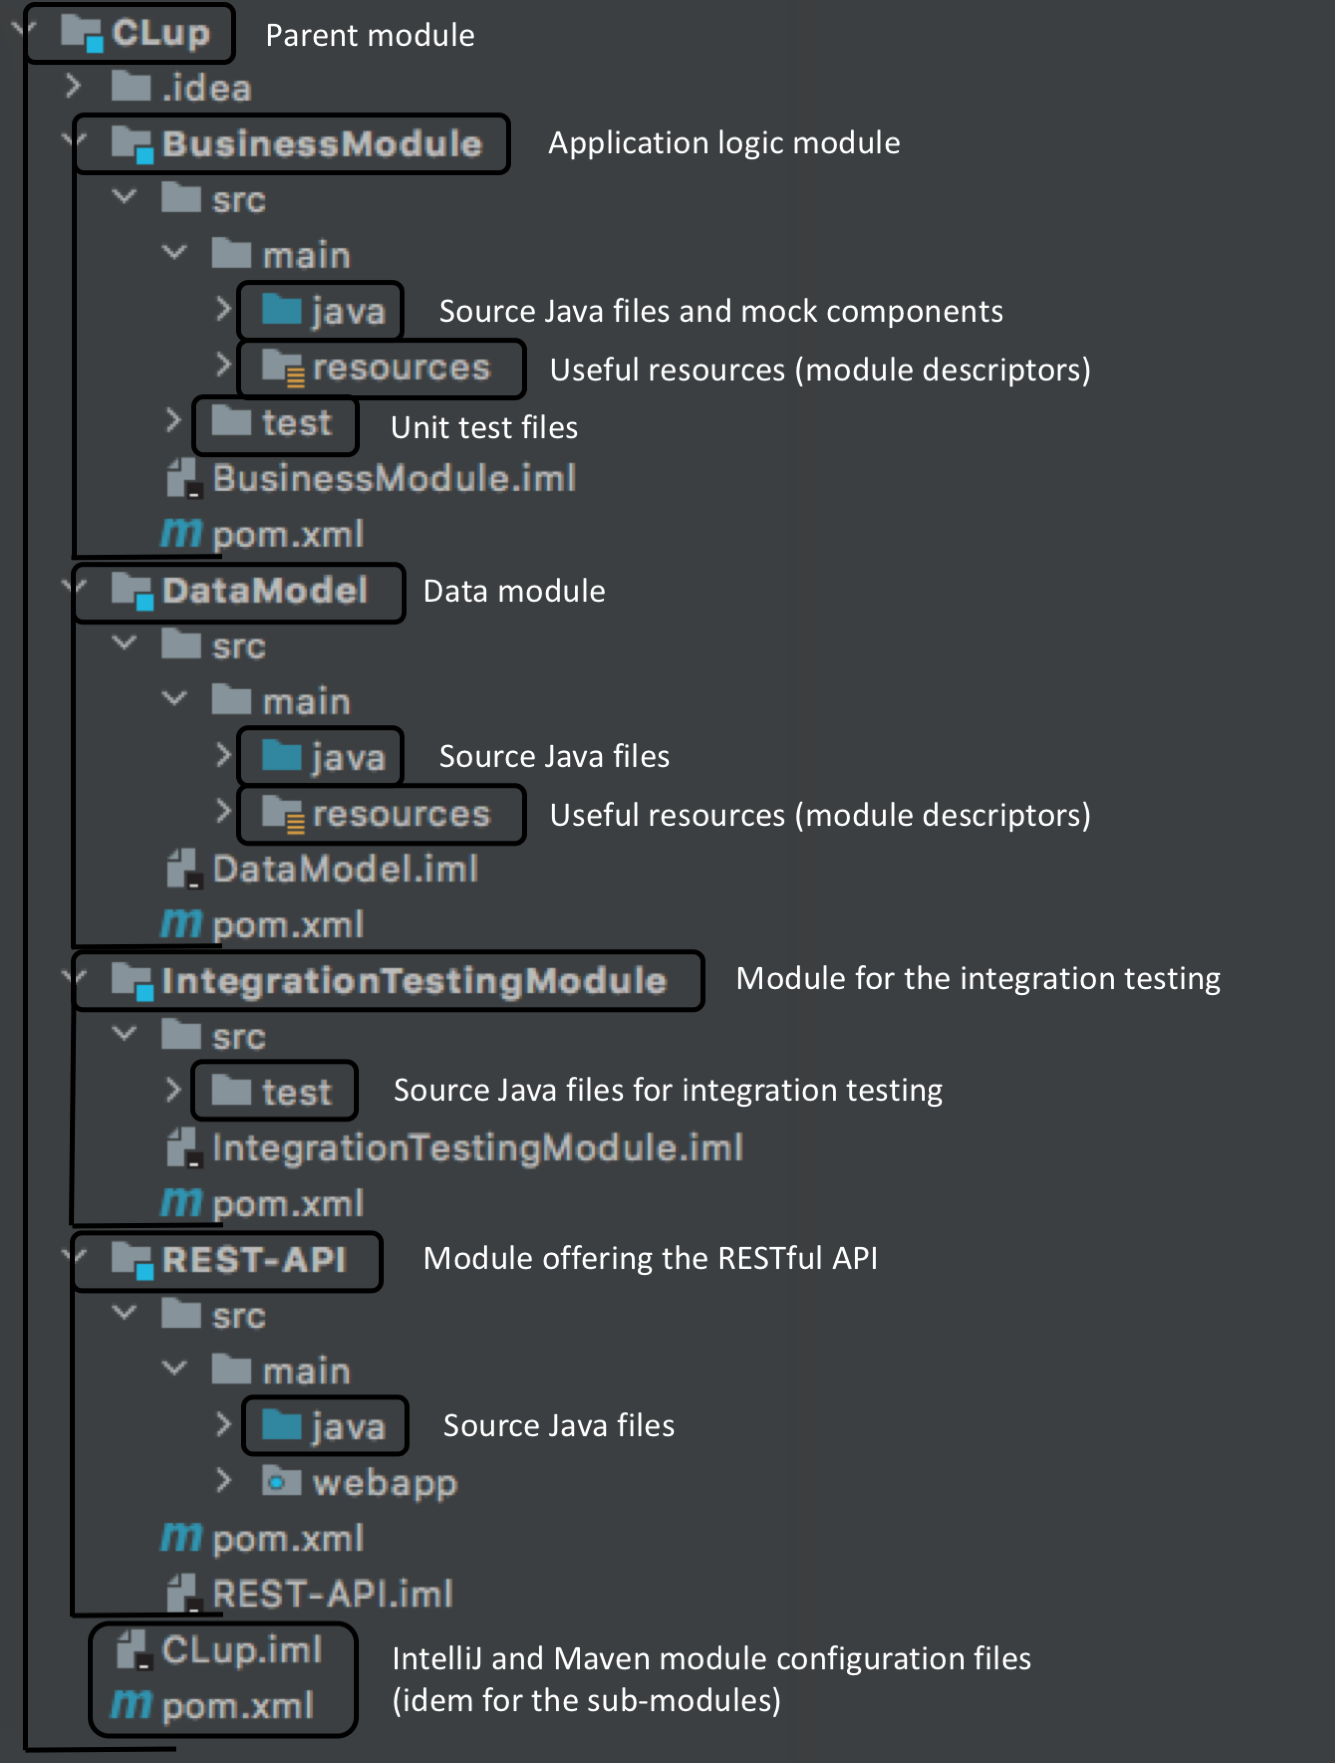
\includegraphics[width=.8\textwidth, height=\textheight, keepaspectratio]{pictures/codestructure_java.png}
        \caption{Code structure of the Java Server}
        \label{figure:codestructure_java}
    \end{figure}
    

\chapter{Testing}
    Following the testing plan outlined in the DD,  the testing phase consisted in the unit testing and the integration testing process. At the end of these tests, a deep end-to-end system test of the functions included in the prototype has been performed, simulating the typical user interactions with the mobile application.
    
    \section{Server Unit test}
    The purpose of unit tests is to verify the correctness of the algorithms and the code implemented in the component under test. The de-facto standard for executing these kinds of tests on Java is the JUnit framework, which allows to perform repeatable tests, checking for the correct execution of the given test code. \par
    Fundamental characteristic of unit tests is the possibility to test the code in isolation and limiting as much as possible side effect situations. This in order to avoid the unpleasant situation in which the execution of the tests leads the entire component under test in a state of inconsistency. \par
    Unit tests have been performed on the most significant functionalities of the prototype components. In order to achieve the expected results, the Mockito framework has been exploited to run unit tests whenever required. Indeed, Mockito allows to generate mock objects of the needed class, thanks to the method mock(Class), and to simulate the mocked object methods, if needed. The mock extends the class that the component under test requires to correctly work, exposing the same interface of the simulated class. In this way, it is possible to ignore the fact that we are dealing with a mock object. An example of this behaviour can be found in each unit test: since EJBs injection is not performed during the JUnit execution and since all the components interact with the DataModel, this last component has been mocked. Its methods’ behavior is simulated whenever needed, thanks to the \texttt{when(dataModel.method()).then(doSomething)} Mockito method. \par
    Moreover, in order to manually inject the mocked DataModel bean in each of the different beans under test, specific classes have been designed, which extend the real ones, placed under the package \texttt{it.polimi.se2.ricciosorrentinotriuzzi.business.components.mockcomponents} in the BusinessModule. 
    
    \section{Server and Database Integration Test}
    Integration test is a fundamental test phase in which components interacting with other ones are tested together, in order to check whether their interaction has been designed properly. To do so, the JUnit and Mockito frameworks have been used to test these interactions, mocking absent components when needed, as in the case of the integration test between the RequestHandler, the DataModel and Database. \par
    Tests are performed in the IntegrationModule, a module defined ad-hoc for the integration testing, which depends on both the DataModule and the BusinessModule, that is not included in the CLup deployed artifact and which contains the classes specifying each test. Moreover, a new class that extends the DataModel one has been defined, called “DataModelMock”, that facilitates the execution of the integration testing. \par
    Since all the following specified tests involve the database, a correct initialization of its state is required in the setup method of each of them, executed by JUnit before every single test. This is done by starting a new JPA transaction and invoking the dbInit method of the DataModelMock, which initializes the database, emptying all its tables. Then, the database is populated with the instances of the entities involved in each test, generated ad-hoc in the setup method. \par
    Finally, after the execution of each of them, the transaction is rolled back in order to not affect the real data in the database.

    \newpage
    \subsection{I1 - VisitManager and DataModel}
    \begin{figure}[H]
        \centering
        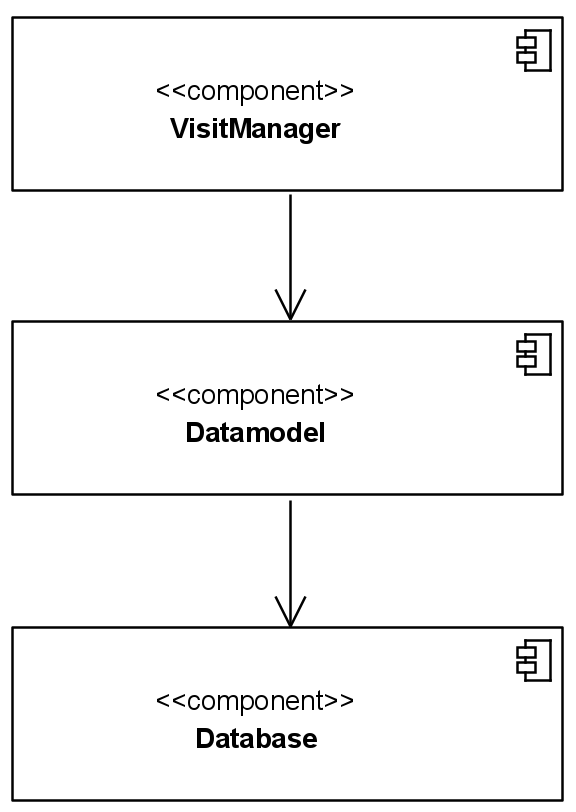
\includegraphics[width=.5\textwidth, height=\textheight, keepaspectratio]{pictures/integration_diagrams/integration_visitmanager_datamodel.png}
        \caption{VisitManager, DataModel and Database integration test}
        \label{figure:integration_visitmanager_datamodel}
    \end{figure}
    \begin{longtable}[c]{|>{\bfseries{}}c|H{.5\textwidth}|}
        \hline
        Test Group ID & I1 - VisitManager and DataModel \\ \hline
        Server Subcomponents & VisitManager, DataModel \\ \hline
        Description & Group of tests to check the interactions between the VisitManager and the DataModel \\ \hline
        Environmental needs & The DataModel and the database are working properly \\ \hline
        \caption{Test Group I1 - Visit Manager and DataModel}
        \label{table:test_I1}
    \end{longtable}
    
    \newpage
    \subsubsection{Validate Access}
    \begin{longtable}[c]{|>{\bfseries{}}c|H{.5\textwidth}|}
        \hline
        Test ID & I1.1 - Validate access \\ \hline
        Server Subcomponents & VisitManager, DataModel \\ \hline
        Input Specification & Invocation of the \texttt{validateAccess} method from the AccessControl API, specifying a visit token and a store ID \\ \hline
        Output Specification & Check whether the number of people allowed to enter is equal to the one specified in the request if it is in ready state, zero otherwise \\ \hline
        Description & The test is focused on verifying the acceptance of a request for accessing its specified store. The VisitManager invokes the \texttt{checkReadyRequest} method of the DataModel, which queries the database returns the number of people allowed to enter the store if the request is in ready state, zero otherwise \\ \hline
        \caption{Test I1.1 - Validate access}
        \label{table:test_I1.1}
    \end{longtable}
    
    \subsubsection{Validate exit}
    \begin{longtable}[c]{|>{\bfseries{}}c|H{.5\textwidth}|}
        \hline
        Test ID & I1.2 - Validate exit \\ \hline
        Server Subcomponents & VisitManager, DataModel \\ \hline
        Input Specification & Invocation of the \texttt{validateExit} method from the AccessControl API, specifying a visit token and a store ID \\ \hline
        Output Specification & Check whether the number of people allowed to exit is equal to the one specified in the request if it is in fulfilled state, zero otherwise \\ \hline
        Description & The test is focused on verifying the acceptance of a request for exiting its specified store. The VisitManager invokes the \texttt{validateExit} method of the DataModel, which queries the database returns the number of people allowed to exit the store if the request is in fulfilled state, zero otherwise \\ \hline
        \caption{Test I1.2 - Validate exit}
        \label{table:test_I1.2}
    \end{longtable}
    
    \subsubsection{Confirm access}
    \begin{longtable}[c]{|>{\bfseries{}}c|H{.5\textwidth}|}
        \hline
        Test ID & I1.3 - Confirm access \\ \hline
        Server Subcomponents & VisitManager, DataModel \\ \hline
        Input Specification & Invocation of the \texttt{confirmAccess} method from the AccessControl API, specifying a visit token, the number of people entering the store and the store ID \\ \hline
        Output Specification & Check if the store occupancy is correctly increased, if the request status is ``fulfilled", its “number of people” field is correctly updated and if the visit starting time is correctly set \\ \hline
        Description & The VisitManager invokes the \texttt{startVisit} method of the DataModel, which queries the database and, if the request is in ready state, modifies it in ``fulfilled", correctly updates the number of people specified in the request if needed and increases the occupancy of the store \\ \hline
        \caption{Test I1.3 - Confirm access}
        \label{table:test_I1.3}
    \end{longtable}
    
    \subsubsection{Confirm exit}
    \begin{longtable}[c]{|>{\bfseries{}}c|H{.5\textwidth}|}
        \hline
        Test ID & I1.4 - Confirm access \\ \hline
        Server Subcomponents & VisitManager, DataModel \\ \hline
        Input Specification & Invocation of the \texttt{confirmExit} method from the AccessControl API, specifying a visit token, the number of people exiting the store and the store ID \\ \hline
        Output Specification & Check if the store occupancy is correctly decreased, if the request status is ``completed" and if the visit completion time is correctly set \\ \hline
        Description & The VisitManager invokes the \texttt{endVisit} method of the DataModel, which queries the database and, if the request is in fulfilled state, modifies it in ``completed" and decreases the occupancy of the store \\ \hline
        \caption{Test I1.4 - Confirm exit}
        \label{table:test_I1.4}
    \end{longtable}
    
    \subsubsection{New request}
    \begin{longtable}[c]{|>{\bfseries{}}c|H{.5\textwidth}|}
        \hline
        Test ID & I1.5 - New request \\ \hline
        Server Subcomponents & VisitManager, DataModel \\ \hline
        Input Specification & Invocation of the \texttt{newRequest} method from the RequestHandler, which informs that a new visit request has been placed \\ \hline
        Output Specification & In case of a Line-up request, it checks that the request is in: 
        \begin{itemize}
            \item ready state if the customer can immediately enter the store, since the current occupancy would not exceed its maximum;
            \item pending state, otherwise.
        \end{itemize}
        In case of a Booking request, it performs the same check when the specified desired time of entrance comes \\ \hline
        Description & In case of Line-up requests, the visit manager immediately checks if the store would exceed its maximum occupancy if the request was in ready state. If not so, then it invokes the \texttt{allowVisitRequest} of the DataModel, that in case of line-ups also updates their estimated time of entrance. \par 
        The same job is scheduled to be performed when the specified desired time of entrance comes in case of booking requests \\ \hline
        \caption{Test I1.5 - New request}
        \label{table:test_I1.5}
    \end{longtable}
    
    
    \newpage
    \subsubsection{Check new ready request}
    \begin{longtable}[c]{|>{\bfseries{}}c|H{.5\textwidth}|}
        \hline
        Test ID & I1.6 - Check new ready request \\ \hline
        Server Subcomponents & VisitManager, DataModel \\ \hline
        Input Specification & Invocation of the \texttt{checkNewReadyRequest} method from the RequestHandler when a customer deletes a pending or ready request, and from the VisitManager itself when a customer exits the store \\ \hline
        Output Specification & It checks whether all the requests that can enter the store without exceeding its maximum occupancy are set in ready state, following the access policies specified in the RASD and DD \\ \hline
        Description & The DataModel is asked by the VisitManager to query the database in order to retrieve all the pending bookings that should be allowed to enter the store. Then the VisitManager determines which of them can actually enter the store, and asks the DataModel to set them in ready state. Then, if there is space available in the store in terms of current occupancy, the same job is performed over pending line-up requests \\ \hline
        \caption{Test I1.6 - Check new ready request}
        \label{table:test_I1.6}
    \end{longtable}
    
    \subsection{I2 - RequestHandler and DataModel}
    \begin{figure}[H]
        \centering
        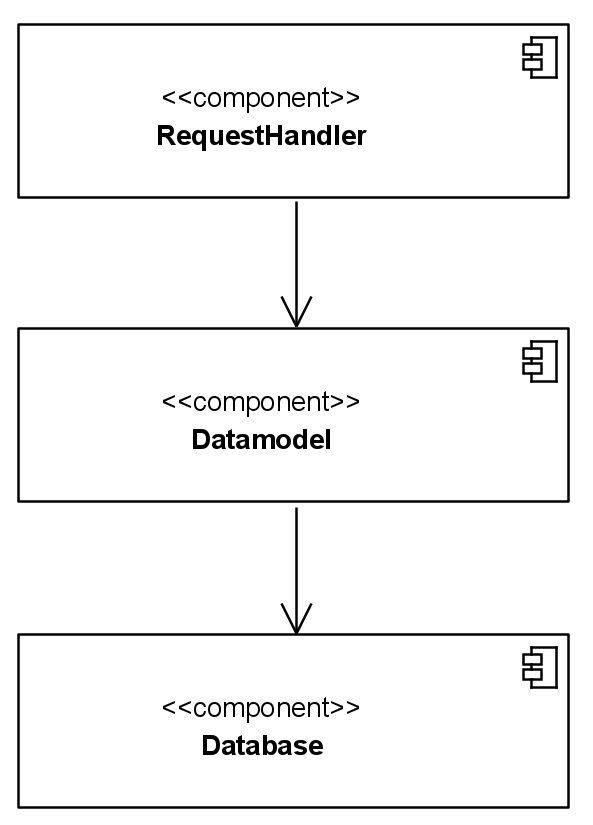
\includegraphics[width=.5\textwidth, height=\textheight, keepaspectratio]{pictures/integration_diagrams/integration_requesthandler_datamodel.png}
        \caption{RequestHandler, DataModel and Database integration test}
        \label{figure:integration_requesthandler_datamodel}
    \end{figure}
    
    \begin{longtable}[c]{|>{\bfseries{}}c|H{.5\textwidth}|}
        \hline
        Test Group ID & I2 - RequestHandler and DataModel \\ \hline
        Server Subcomponents & RequestHandler, DataModel \\ \hline
        Description & Group of tests to check the interactions between the RequestHandler and the DataModel \\ \hline
        Environmental needs & The DataModel and the database are working properly. The interactions between the RequestHandler and the VisitManager are not considered during the test \\ \hline
        \caption{Test Group I2 - RequestHandler and DataModel}
        \label{table:test_I2}
    \end{longtable}
    
    \newpage
    \subsubsection{Line-up}
    \begin{longtable}[c]{|>{\bfseries{}}c|H{.5\textwidth}|}
        \hline
        Test ID & I2.1 - Line-up \\ \hline
        Server Subcomponents & RequestHandler, DataModel \\ \hline
        Input Specification & Invocation of the \texttt{line-up} method from the LineUp interface when a customer requests to line-up for a store \\ \hline
        Output Specification & Checks that the request is rejected if:
        \begin{itemize}
            \item The number of people specified in the request is not strictly positive or exceeds the store maximum occupancy;
            \item The store is closed;
            \item The customer has already made a line-up request for any of the available stores.
        \end{itemize}
        Checks that the request is accepted if:
        \begin{itemize}
            \item The number of people specified in the request  does not exceed the store maximum occupancy, the store is open and the customer is not already in line for any available store.
        \end{itemize} \\ \hline
        Description & The number of people specified in the request does not exceed the store maximum occupancy, the store is open and the customer is not already in line for any available store \\ \hline
        \caption{Test I2.1 - Line-up}
        \label{table:test_I2.1}
    \end{longtable}
    
    \newpage
    \subsubsection{Booking}
    \begin{longtable}[c]{|>{\bfseries{}}c|H{.5\textwidth}|}
        \hline
        Test ID & I2.2 - Booking \\ \hline
        Server Subcomponents & RequestHandler, DataModel \\ \hline
        Input Specification & Invocation of the \texttt{book} method from the Booking interface when a customer request to book a visit for a store \\ \hline
        Output Specification & The request is rejected if:
        \begin{itemize}
            \item The customer is not an app customer;
            \item The customer has already booked a visit (possibly to another store) that overlaps with the specified desired time-interval;
            \item The store is closed during the specified time interval;
            \item The number of people specified in the request is not strictly positive or is greater than the store maximum occupancy;
            \item The desired time-interval begins before the end of the current estimated queue disposal time of the selected store;
            \item The current occupancy of the store is already maximized by others’ booking requests in the specified time interval;
            \item The current occupancy of one of the specified store’s product sections, if any, is already maximized by others’ booking requests in the specified time interval.
        \end{itemize}
        The request is accepted if:
        \begin{itemize}
            \item  During the desired time-interval the customer does not have other bookings, the store does not exceed its maximum occupancy, and the store is open.
        \end{itemize} \\ \hline
        Description & The RequestHandler asks the DataModel to retrieve the store and customer information from the database. Then, it checks if the  customer is an app customer, that the store is open across the specified time interval and if the specified number of people is consistent with the previously mentioned constraints. Then the RequestHandler invokes the DataModel in order to query the Database and retrieve the updated current queue disposal time, and so checks if the desired starting time is past it. Then, the RequestHandler asks the DataModel to retrieve from the Database the bookings already placed by the customer, and if none of them is found, also to retrieve all the bookings placed by other customers for the selected store in the selected time interval. If occupancy constraints are satisfied, then the request is accepted and the DataModel is asked to persist it on the Database. \\ \hline
        \caption{Test I2.2 - Booking}
        \label{table:test_I2.2}
    \end{longtable}
    
    \subsection{I3 - CustomerController and DataModel}
    \begin{figure}[H]
        \centering
        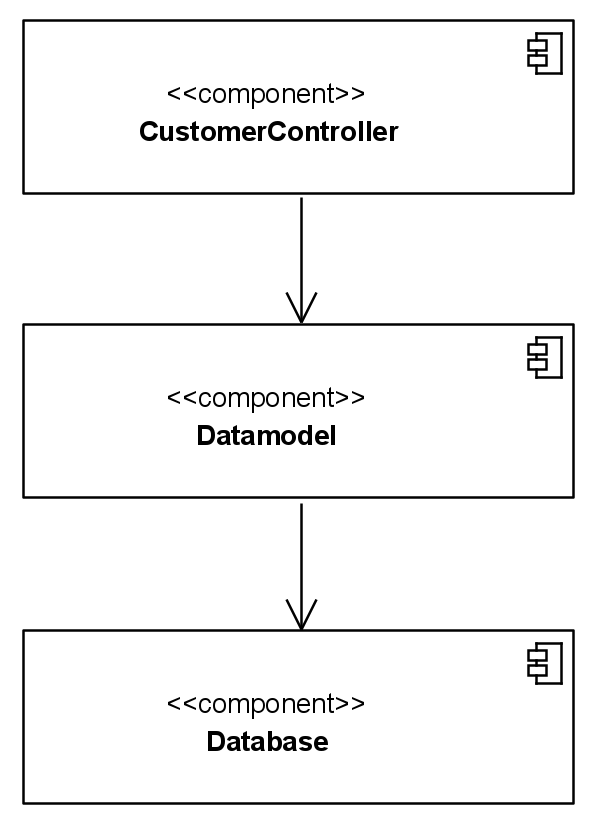
\includegraphics[width=.5\textwidth, height=\textheight, keepaspectratio]{pictures/integration_diagrams/integration_customercontroller_datamodel.png}
        \caption{VisitManager, DataModel and Database integration test}
        \label{figure:integration_customercontroller_datamodel}
    \end{figure}
    
    \begin{longtable}[c]{|>{\bfseries{}}c|H{.5\textwidth}|}
        \hline
        Test Group ID & I3 - CustomerController and DataModel \\ \hline
        Server Subcomponents & CustomerController, DataModel \\ \hline
        Description & Testing the interactions between the RequestHandler and the DataModel \\ \hline
        Environmental needs & The DataModel and the database are working properly \\ \hline
        \caption{Test Group I3 - CustomerController and DataModel}
        \label{table:test_I3}
    \end{longtable}
    
    \newpage
    \subsubsection{Customer's active line-up requests}
    \begin{longtable}[c]{|>{\bfseries{}}c|H{.5\textwidth}|}
        \hline
        Test ID & I3.1 - Customer's active line-up requests \\ \hline
        Server Subcomponents & CustomerController, DataModel \\ \hline
        Input Specification & Invocation of the method \texttt{getCustomerActiveLineups} from the Customer Interface when a customer asks to retrieve its active line-up requests \\ \hline
        Output Specification & Checks if each line-up request obtained by querying the database is active \\ \hline
        Description & The CustomerController asks the DataModel to query the Database in order to retrieve the active line-up requests of the specified customer \\ \hline
        \caption{Test I3.1 - Customer's active line-up requests}
        \label{table:test_I3.1}
    \end{longtable}
    
    \subsubsection{Customer's active bookings}
    \begin{longtable}[c]{|>{\bfseries{}}c|H{.5\textwidth}|}
        \hline
        Test ID & I3.2 - Customer's active bookings \\ \hline
        Server Subcomponents & CustomerController, DataModel \\ \hline
        Input Specification & Invocation of the method \texttt{getCustomerActiveBookings} from the Customer Interface when a customer asks to retrieve its active booking requests \\ \hline
        Output Specification & Checks whether each booking of the customer obtained by querying the database is active \\ \hline
        Description & The CustomerController asks the DataModel to query the Database in order to retrieve the active booking requests of the specified customer \\ \hline
        \caption{Test I3.2 - Customer's active bookings}
        \label{table:test_I3.2}
    \end{longtable}
    
    \subsection{I4 - StoreStatusHandler and DataModel}
    \begin{figure}[H]
        \centering
        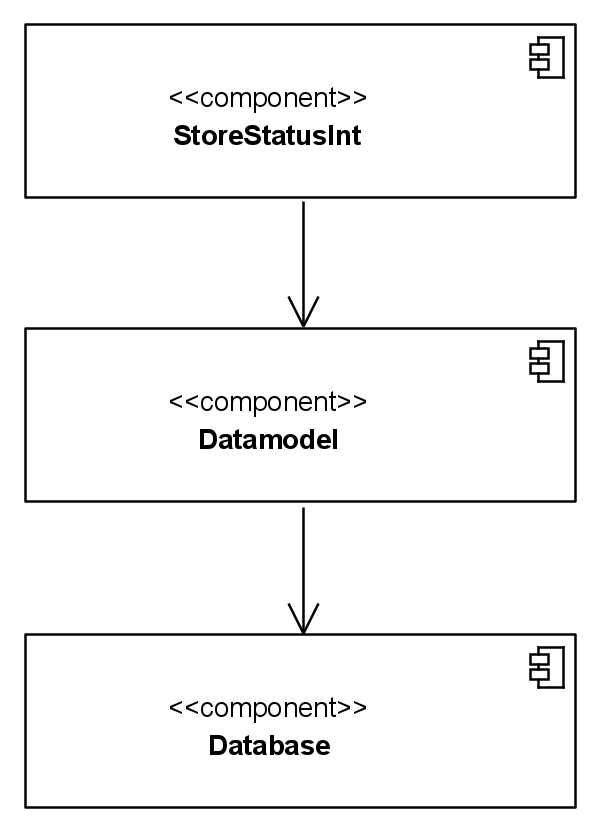
\includegraphics[width=.5\textwidth, height=\textheight, keepaspectratio]{pictures/integration_diagrams/integration_storestatushandler_datamodel.png}
        \caption{StoreStatusHandler, DataModel and Database integration test}
        \label{figure:integration_storestatushandler_datamodel}
    \end{figure}
    
    \begin{longtable}[c]{|>{\bfseries{}}c|H{.5\textwidth}|}
        \hline
        Test Group ID & I4 - StoreStatusHandler and DataModel \\ \hline
        Server Subcomponents & StoreStatusHandler, DataModel \\ \hline
        Description & Testing the interactions between the StoreStatusHandler and the DataModel \\ \hline
        Environmental needs & The DataModel and the database are working properly \\ \hline
        \caption{Test Group I3 - CustomerController and DataModel}
        \label{table:test_I3}
    \end{longtable}
    
    
    \newpage
    \subsubsection{Store general info}
    \begin{longtable}[c]{|>{\bfseries{}}c|H{.5\textwidth}|}
        \hline
        Test ID & I4.1 - Store general info \\ \hline
        Server Subcomponents & StoreStatusHandler, DataModel \\ \hline
        Input Specification & The StoreStatusHandler is asked via the StoreInfoInterface to provide the specified store’s information \\ \hline
        Output Specification & Checks whether the information obtained from the DataModel is compliant with the test store created and persisted appositely before the test \\ \hline
        Description & The StoreStatusHandler asks the DataModel to get retrieve the information about the specified store from the database \\ \hline
        \caption{Test I4.1 - Store general info}
        \label{table:test_I4.1}
    \end{longtable}
    
    
    \subsubsection{Get chains and autonomous stores}
    \begin{longtable}[c]{|>{\bfseries{}}c|H{.5\textwidth}|}
        \hline
        Test ID & I4.2 - Get chains and autonomous stores \\ \hline
        Server Subcomponents & StoreStatusHandler, DataModel \\ \hline
        Input Specification & The StoreStatusHandler is asked via the StoreInfoInterface to provide the list of chains and autonomous store, and to restrict the selection to the ones in the specified city, if any \\ \hline
        Output Specification & Checks whether the information obtained from the DataModel is compliant with the test stores and the chains created and persisted appositely before the test \\ \hline
        Description & The StoreStatusHandler asks the DataModel to get the distinct chains and autonomous stores of the specified city (if any, all of them otherwise) from the database \\ \hline
        \caption{Test I4.2 - Get chains and autonomous stores}
        \label{table:test_I4.2}
    \end{longtable}
    
    \newpage
    \subsubsection{Get chain’s stores}
    \begin{longtable}[c]{|>{\bfseries{}}c|H{.5\textwidth}|}
        \hline
        Test ID & I4.3 - Get chain’s stores \\ \hline
        Server Subcomponents & StoreStatusHandler, DataModel \\ \hline
        Input Specification & The StoreStatusHandler is asked via the StoreInfoInterface to provide the list of stores of a given chain, and to restrict the selection to the ones in the specified city, if any \\ \hline
        Output Specification & Checks whether the information obtained from the DataModel is compliant with the test stores and the chains created and persisted appositely before the test \\ \hline
        Description & The StoreStatusHandler asks the DataModel to get the stores of a specific chain. If a city is specified, the DataModel gets only the stores in that city of the specified chain \\ \hline
        \caption{Test I4.3 - Get chain’s stores}
        \label{table:test_I4.3}
    \end{longtable}
    

\chapter{Installation instructions}
    The following instructions are intended to let the reader reach a configuration as close as possible to the one used during the software development and testing. Even if other configurations might work as well, the correct operation of the application is not guaranteed. \par
    As a prerequisite, a Mac running macOS Catalina 10.15.4 or later is required in order to simulate the mobile iOS application. \par
    Through all the instructions, it’s assumed that the GitHub repository has already been cloned on the target machine(s). \par
    Check that all the devices used are under the same Local Area Network (otherwise it is needed to configure the software accordingly, which is out of the purpose of this section) and that no firewall is blocking connections between the devices.
    \begin{figure}[H]
        \centering
        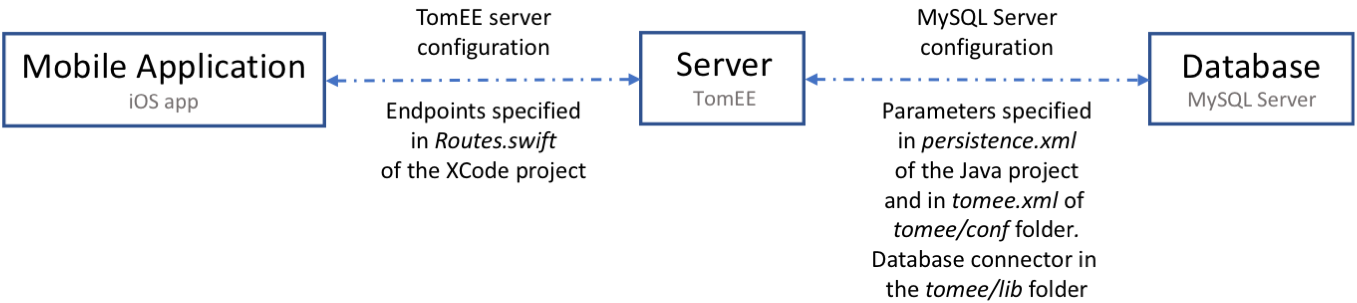
\includegraphics[width=\textwidth, height=\textheight, keepaspectratio]{pictures/interactions.png}
        \caption{Configuration preview}
        \label{figure:interactions}
    \end{figure}
    
    \section{Database}
    As already stated in the DD, it has been chosen a relational database to persist data. The DBMS used is MySQL, available for free for all the major operating systems. Download and install both MySQL Server and MySQL Workbench. Be sure to install an 8.x version. At the time of writing, version 8.0.23 has some issues running on MacOS, which are not related to this project. \par
    The configuration used during the developing and testing of the software is the following:
    \begin{itemize}
        \item Macbook running macOS Catalina 10.15.7;
        \item MySQL Server 8.0.22;
        \item MySQL Workbench 8.0.22.
    \end{itemize}
    Through the installation setup of the server, configure it with the following parameters:
    \begin{itemize}
        \item Port number: \textit{3306};
        \item Default username: \textit{root};
        \item Root password: \textit{EmaGiaVin123}
    \end{itemize}
    If MySQL is already installed and/or configured in a different way, it doesn’t matter: just edit tomee.xml in tomee/conf and the \texttt{persistence.xml} file of the server DataModel module (see the following section). However, they must be changed anyway if the server is hosted by another machine, putting the local IP address of the machine hosting MySQL Server. Then:
    \begin{itemize}
        \item Open MySQL Workbench and connect to the local server;
        \item Go under the Server menu and choose Data Import;
        \item Use the option which allows the import from a self-contained file;
        \item Select the dump provided in Implementation/Database of our GitHub repo;
        \item Add a new schema \texttt{clup\_db} as the default target schema;
        \item Start import by clicking on the homonym button on the bottom right.
    \end{itemize}

    \section{CLup Server}
    The CLup business tier has been developed using Java Enterprise Edition. IntelliJ IDEA Ultimate is the IDE used during the development, available for free (30-day evaluation period, free for students) for all the major platforms. The configuration used for the development and testing is the following:
    \begin{itemize}
        \item Macbook running macOS Catalina 10.15.7;
        \item IntelliJ IDEA Ultimate Edition 2020.2.3;
        \item Oracle OpenJDK 15 (can be downloaded from IntelliJ IDEA);
        \item Maven 3.6.3 (included in IntelliJ IDEA);
        \item Apache TomEE plume 8.0.4 (provided in the repo);
        \item MySQL Connector 8.0.21 (included in the provided tomee/lib folder);
    \end{itemize}
    In order to only run the application server, assuming that OpenJDK 15 is already installed and configured, it is only needed to run Apache TomEE. For UNIX-based systems, use the terminal to navigate to the bin folder inside the provided tomee folder and execute \texttt{./catalina.sh run}.
    In order to prepare a suitable workstation for inspecting, running and testing this part of the software, do the following steps:
    \begin{itemize}
        \item Download IntelliJ IDEA Ultimate from the official website and install it;
        \item Run IntelliJ IDEA and open the project selecting the Implementation/JavaServer/CLup folder;
        \item Wait until all the dependencies are automatically downloaded by Maven (take a look on the right part of the bottom bar);
        \item Go to File > Project Structure > Project (on the side bar). Check that under the section Project SDK it is selected OpenJDK 15 (if not available download and install it by clicking on the relative option of the dropdown menu);
        \item Configure the application server in IntelliJ IDEA by clicking on Run menu > Edit configuration. Add a TomEE configuration by clicking on the add button (+) and selecting a Local instance of TomEE Server. Click on “Configure” on the upper-right corner and select the provided tomee folder as TomEE Home. Then confirm by clicking on OK. In the deployment tab click on the add button (+) in the “Deploy at the server startup” box and select the CLup artifact (check that the application context is /CLup). Click on OK;
        \item Run the application by clicking on the play button on the toolbar.
    \end{itemize}
    As stated in the instructions for the database installation, \textit{tomee.xml} in \textit{tomee/conf} and the \textit{persistence.xml} file of the DataModel module (available under \textit{src/main/resources} of that module), must reflect the database configuration. \par
    Furthermore, be sure that no other server is running on port 8080, which is the one used by TomEE, otherwise it will throw an error during its execution.

    \section{iOS Customer Mobile application}
    Since the customer mobile application developed has an iOS device as target, XCode is required to build the application and to test it on a real device or on the simulator included in XCode. An Apple Development Account is needed (it is free and available for every Apple ID). The mobile application has iOS 14.x as target OS. \par
    Thus, a version of XCode which supports iOS 14 is required. The configuration used for developing and testing the application is the following:
    \begin{itemize}
        \item XCode 12.4 (requires macOS Catalina 10.15.4 or later for an Intel-based Mac, or macOS Big Sur 11 or later for an Apple Silicon based Mac);
        \item iPhone 11 with iOS 14.4, through the simulator;
        \item iPad Air 2 with iOS 14.4.
    \end{itemize}
    XCode can be installed from the Mac App Store. If XCode was never installed before, go to Xcode \texttt{Menu > Preferences > Accounts tab}. Then add your Apple Developer Account (basically logging in with your Apple ID) by clicking on the add button on the bottom left. Then open the XCode project file (\texttt{CLup.xcodeproj}), go to CLup project (the root element), click on the target element of the left bar and select the \texttt{Signing > Capabilities} tab. Under the team section, select your \textit{Personal Team}. Change the bundle identifier if the error “\textit{Failed to register bundle identifier}” appears. \par
    Before running it, the reader must modify the address and the port of the server endpoint according to the server configuration. The attribute \texttt{baseURL} of the file \texttt{Routes.swift} available under the project tree is what should be edited. If the previous instructions have been followed, overwrite the \texttt{baseURL} string with “\texttt{http://<SERVER\_IP>:8080/CLup}”, where \texttt{<SERVER\_IP>} is the local IP address of the machine hosting the server. If the server is running on the same machine and no physical device is going to be used, simply write localhost instead of \texttt{<SERVER\_IP>}. \par
    Note that if the TomEE port has been changed, one must overwrite 8080 with the chosen port. \par
    Finally, it only requires to select the target device in the upper toolbar and click on run. \par
    Due to Apple security policy, when testing on a real device, on the first launch of the CLup mobile application it is needed to trust the developer. To do so, go under \texttt{
    Settings > Generals > Device Management > Apple Development > Trust}. \par
    Then restart the app.

    \section{iOS AMS Simulator}
    In order to test the accesses and exits of customers to a store, the team also developed a test iOS application to simulate the behaviour of the Access Management System of a store. It requires a real device since it uses the device’s camera to scan the QR code which identifies the visit request. If not available, one can always simulate it by manually interacting with the RESTful API.  \par
    As for the customer mobile application, XCode is required to build the application and to test it on a real device. The AMS Simulator has iOS 13.x as target OS. \par
    Thus, a version of XCode which supports iOS 13 is required. The configuration used for developing and testing the application is the following:
    \begin{itemize}
        \item XCode 12.4 (requires macOS Catalina 10.15.4 or later for an Intel-based Mac, or macOS Big Sur 11 or later for an Apple Silicon based Mac);
        \item iPad Air 2 with iOS 14.4.
    \end{itemize}
    The installation and setup procedure is the same of the iOS customer mobile application. 

\chapter{Effort spent}
    All the members of the group worked mainly together, in order to guarantee consistency through the entire document. Each member of the group spent approximately 45 hours doing team working. In addition to team working, individual work has been partitioned as shown in the following tables:
    \subsubsection{Riccio Vincenzo}
    \begin{longtable}[c]{|H{.55\textwidth}|c|}
        \hline
        \textbf{Section} & {\bfseries{Hours}} \\ \hline
        \textbf{Team working} & \textbf{20} \\ \hline
        iOS Customer Mobile Application implementation                                  & 17 \\ \hline
        AMS Simulator implementation   & 3 \\ \hline
        Server implementation                          & 8 \\ \hline
        Database definition                         & 0 \\ \hline
        Server unit testing                         & 0 \\ \hline
        Server integration testing                           & 2 \\ \hline
        End-to-end testing                      & 5 \\ \hline
        \LaTeX                                 & 0 \\ \hline
        \caption{Effort spent -- Riccio Vincenzo}
        \label{table:effort_riccio}
    \end{longtable}
    
    \newpage
    \subsubsection{Sorrentino Giancarlo}
    \begin{longtable}[c]{|H{.55\textwidth}|c|}
        \hline
        \textbf{Section} & {\bfseries{Hours}} \\ \hline
        \textbf{Team working} & \textbf{20} \\ \hline
        iOS Customer Mobile Application implementation                                  & 0 \\ \hline
        AMS Simulator implementation   & 0 \\ \hline
        Server implementation                          & 16 \\ \hline
        Database definition                         & 2 \\ \hline
        Server unit testing                         & 7 \\ \hline
        Server integration testing                           & 8 \\ \hline
        End-to-end testing                      & 2 \\ \hline
        \LaTeX                                 & 0 \\ \hline
        \caption{Effort spent -- Sorrentino Giancarlo}
        \label{table:effort_sorrentino}
    \end{longtable}
    
    \subsubsection{Triuzzi Emanuele}
    \begin{longtable}[c]{|H{.55\textwidth}|c|}
        \hline
        \textbf{Section} & {\bfseries{Hours}} \\ \hline
        \textbf{Team working} & \textbf{20} \\ \hline
        iOS Customer Mobile Application implementation                                  & 3 \\ \hline
        AMS Simulator implementation   & 0 \\ \hline
        Server implementation                          & 11 \\ \hline
        Database definition                         & 4 \\ \hline
        Server unit testing                         & 4 \\ \hline
        Server integration testing                           & 4 \\ \hline
        End-to-end testing                      & 5 \\ \hline
        \LaTeX                                 & 4 \\ \hline
        \caption{Effort spent -- Triuzzi Emanuele}
        \label{table:effort_triuzzi}
    \end{longtable}

\chapter{References}
    This chapter contains references to the tools and resources used during the writing of the document. \par
    \begin{itemize}
        \item \textit{GitHub} 
        
        \url{https://github.com/SirGian99/RiccioSorrentinoTriuzzi}
        \item \textit{TomEE} 
        
        \url{https://tomee.apache.org/}
        \item \textit{IntelliJ IDEA} 
        
        \url{https://www.jetbrains.com/idea}
        \item \textit{Apache Maven} 
        
        \url{https://maven.apache.org/guides/}
        \item \textit{Apple Swift} 
        
        \url{https://developer.apple.com/swift/}
        \item \textit{Apple SwiftUI} 
        
        \url{https://developer.apple.com/xcode/swiftui/}
        \item {\textit{SwiftyJSON}} 
        
        \url{https://github.com/SwiftyJSON/SwiftyJSON}
        \item \textit{EclipseLink} 
        
        \url{https://www.eclipse.org/eclipselink/}
        \item \textit{JSON Java} 
        
        \url{https://github.com/stleary/JSON-java}
        \item \textit{JUnit} 
        
        \url{https://junit.org/junit5/}

    \end{itemize}

\listoftables
\listoffigures

\end{document}